\documentclass{article}

\usepackage[final,nonatbib]{nips_2016}

\usepackage{url}
\usepackage{amsmath}
\usepackage{booktabs}
\usepackage{hyperref}
\usepackage{amsfonts}
\usepackage{nicefrac}
\usepackage{microtype}
\usepackage[T1]{fontenc}
\usepackage[utf8]{inputenc}
\usepackage[pdftex]{graphicx}
\usepackage[caption=false,font=footnotesize]{subfig}

\graphicspath{{./Images/}}
\DeclareGraphicsExtensions{.pdf,.jpeg,.png}

\title{Data-efficient Motor-skills Learning in Latent Spaces for Robotic Clothing Assistance}

\author{
  Nishanth Koganti$^{1,2}$, Tomoya Tamei$^{1}$, Kazushi Ikeda$^{1}$, Tomohiro Shibata$^{2}$\\
  $^1$ Nara Institute of Science and Technology, Japan~~~$^2$ Kyushu Institute of Technology, Japan\\
  \texttt{\{nishanth-k,tomo-tam,kazushi\}@is.naist.jp, tom@brain.kyutech.ac.jp} \\
}

\begin{document}

\maketitle

\begin{abstract}
Robotic implementation of clothing assistance is a challenging problem that can greatly improve the quality-of-life for the elderly and disabled. In this study, we propose a data-efficient representation to encode task specific motor-skills of the robot using Bayesian nonparametric latent manifold learning. We implement our framework in a practical setting with a dual-arm robot performing clothing tasks. We demonstrate that performing motor-skills learning in such task specific latent spaces outperforms learning in the high-dimensional joint configuration space of the robot. Furthermore, our framework can also be used as a tool for learning from demonstration to impart novel skills to the robot.
\end{abstract}

\section{Introduction}
\label{section:introduction}

Clothing assistance is a necessity in the daily life of the elderly and disabled people. However, robotic clothing assistance is still considered an open problem. Design of a robust framework involves reliable cloth state estimation in real-time and a motor skills learning framework that can detect and adapt to various failure scenarios. Tamei \emph{et al.}~\cite{tamei} proposed a reinforcement learning (RL) framework for clothing assistance with a dual-arm robot to cloth a soft mannequin with a T-shirt initially resting on its arms. For tractable learning time, policy update was done using finite difference policy gradient applied to a single via-point of a single joint in each robot arm. This severely constrained the generalization capability to very different environmental settings such as major changes in the subject's posture or using different clothing article.

To address this problem, we need to consider an alternate representation that is more flexible and suitable for robust learning of motor-skills. An efficient approach is the use of dimensionality reduction (DR) along with reinforcement learning (RL). There have been several studies in this direction in the recent years. Bitzer \emph{et al.}~\cite{bitzer} proposed a learning framework where DR was used as a preprocessing step to extract the problem structure. However, this study relies on a maximum-a-posteriori (MAP) estimate of the latent space and can overfit to the training data. Luck \emph{et al.}~\cite{luck} proposed a policy search framework that inherently combines RL and DR wherein the latent space is learned based on the reward signals. However, this framework relies on the use of linear dimensionality reduction which limits applicability to complex tasks.

In this study, we propose an efficient representation of motor skills that relies on the use of Bayesian Gaussian Process Latent Variable Model (BGPLVM)~\cite{bgplvm}. BGPLVM is capable of learning a data-efficient latent space for clothing tasks performed by a dual-arm robot. Representation of clothing skills in a low-dimensional space enables the use of expressive policy update rules for generalization to very different settings. We apply our proposed method to a clothing assistance setup as shown in Figure~\ref{figure:overview}. We demonstrate that performing policy search in this latent space outperforms learning in the high-dimensional action space. We further present the design of a real-time controller from the BGPLVM latent space that can be used as a tool for Learning from Demonstration (LfD). The experimental results indicate a promising reinforcement learning learning that can be used for challenging tasks such as robotic clothing assistance.

The rest of the paper is structured as follows. The proposed framework is presented in Section~\ref{section:method}. Section~\ref{section:results} includes experimental results and Section~\ref{section:conclusion} concludes the paper with directions for future work.

\section{Proposed Method}
\label{section:method}

\begin{figure}
  \centering
  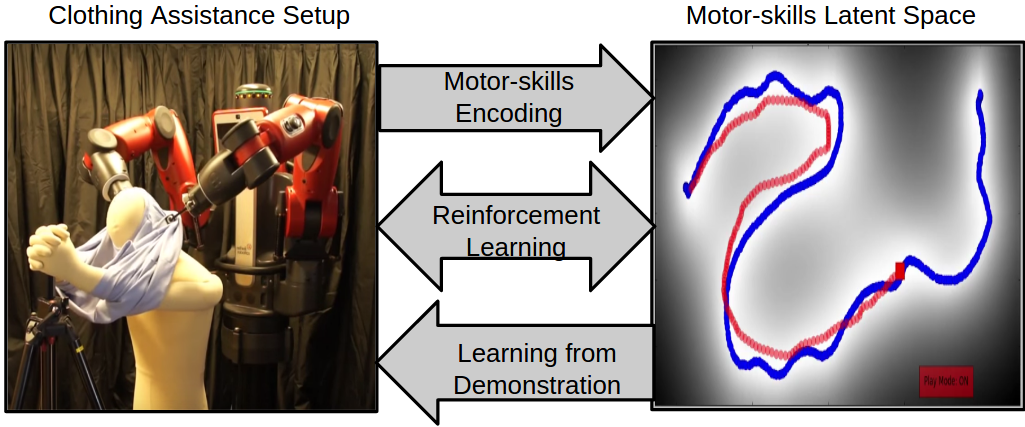
\includegraphics[width=0.8\textwidth]{overview.png}
  \caption{Overview of proposed framework. Figure on the left shows the setup for clothing assistance and the figure on the right shows the latent space encoding the motor skills. This latent space can be used a tool for Learning from Demonstration (LfD) and also for data-efficient reinforcement learning.}
  \label{figure:overview}
\end{figure}
In this study, we explore the suitability of using Bayesian Gaussian Process Latent Variable Model (BGPLVM) to learn a latent space as a low dimensional representation of motor skills for clothing assistance. This section is divided into three parts. Section~\ref{section:bgplvm} provides the formulation of BGPLVM, Section~\ref{section:clothassist} presents the application of BGPLVM in the clothing assistance framework and Section~\ref{section:latentrl} includes the formulation of a policy search framework that relies on the use of this representation.

\subsection{Bayesian Nonparametric Latent Space Learning}
\label{section:bgplvm}

Bayesian Gaussian Process Latent Variable Model (BGPLVM) is a dimensionality reduction technique proposed by Titsias \emph{et al.}~\cite{bgplvm}  derived from the probabilistic model where the observations, $\mathbf{Y} = \{\mathbf{y}_{i} \in \mathbb{R}^D\}_{n=1}^N$, are assumed to be generated from latent inputs $\mathbf{X} = \{\mathbf{x}_{i} \in \mathbb{R}^q\}_{n=1}^N$ through a noisy process,
\begin{equation}
  \mathbf{y}_i = f(\mathbf{x}_i) + \epsilon,~\epsilon \sim \mathcal{N}(\mathbf{0},\beta^{-1}\mathbf{I})
\end{equation}
The mapping function $f$ is modeled using a Gaussian Process (GP) suitable for performing non-linear dimensionality reduction with use of a non-linear kernel function. The marginal likelihood for the generative model is given by:
\begin{equation}
  \label{eqn:marginallikelihood}
  p(\mathbf{Y}|\mathbf{X},\Phi) = \prod_{d=1}^{D} \mathcal{N}(\mathbf{y}_{:,d}|\mathbf{0},\mathbf{K}+\beta^{-1}I)\\
\end{equation}
where $\mathbf{X},\Phi$ are the unknown latent points and hyper parameters for the GP mapping that need to be inferred. $\mathbf{K}$ is the kernel matrix constructed from the latent points. In the generative model, the latent positions need to be marginalized out for having a purely Bayesian treatment. Titsias \emph{et al.}~\cite{bgplvm} proposed a variational inference approach to compute a tractable lower bound for the marginalization thereby inferring a posterior distribution on the latent positions rather than a MAP estimate.

For performing automatic model selection of the latent space dimensionality, the Automatic Relevance Determination (ARD) Kernel can be used in the GP mapping:
\begin{equation}
  \label{eqn:ardkernel}
  k_{\text{ard}}(\mathbf{x}_i,\mathbf{x}_j) = \sigma_{ard}^2~\text{exp}\left( - \frac{1}{2} \sum_{k=1}^q{\alpha_q (x_{i,k} - x_{j,k})^2}\right)
\end{equation}
The ARD weights $\alpha_q$ describe the relevance of each dimension and zero weight indicates complete irrelevance. Maximizing the marginal likelihood w.r.t. these weights allows the inference of latent space dimensionality. The inference for unseen test data can now be performed through a Bayesian formulation instead of relying on a MAP estimation of the latent space. The predictive distribution is given by the ratio of two marginal likelihoods, both of which can be approximated using the variational inference technique:
\begin{equation}
	\label{eqn:testinference}
	p(\mathbf{y}^*|\mathbf{Y}) = \frac{\int p(\mathbf{y}^*,\mathbf{Y}|\mathbf{x}^*,\mathbf{X})p(\mathbf{x}^*,\mathbf{X})d\mathbf{X}d\mathbf{x}^*}{\int p(\mathbf{Y}|\mathbf{X})p(\mathbf{X})d\mathbf{X}}
\end{equation}
Efficient computations to handle test data is further described in \cite{bgplvm}.

\subsection{Motor Skills Representation using BGPLVM}
\label{section:clothassist}

Motor skills for clothing assistance are given by high dimensional joint angle trajectories of the dual-arm robot. The robot also has to maintain several task space constraints such as coupling with a clothing article along with safe human-robot interaction as shown in Figure~\ref{figure:overview}. To address these problems, we propose the use of BGPLVM for learning a low-dimensional latent space through a nonlinear mapping to the kinematic space. The Bayesian treatment avoids over fitting to the training data and automatic inference of latent space dimensionality through the ARD kernel. We consider the clothing task where a dual-arm robot clothes a soft mannequin with a T-shirt which is initially resting on the mannequin's arms. We represent the robot poses in two ways i.e. 1) Kinematic representation given by joint angles $D_K = 14$ and 2) Task space representation given by the end-effector pose of both arms with cartesian position ${P_X,P_Y,P_Z} \in \mathbb{R}^3$ and orientation ${O_X,O_Y,O_Z,O_{\omega}} \in \mathbb{R}^4$ forming a 14-dimensional space $D_T = 14$. We set the dimension of the latent space as $q = 5$, however the dimensionality is eventually inferred through the training of the ARD kernel weights as explained in Section~\ref{section:bgplvm}.

There can be several types of failure scenarios when the robot performs clothing tasks. While clothing, the T-shirt collar could get stuck on the mannequin's head and while unclothing, the T-shirt could get stuck in the mannequin's shoulder joints. To recover from these failures, not only is the trajectory of the robot important, but also the speed of execution. Imparting these skills through kinesthetic movement of the arms can be difficult for a bulky robot and could lead to noisy demonstrations. To address this problem, we have implemented a real-time controller that gets an input signal from the BGPLVM latent space. The BGPLVM model learns a mapping from the low dimensional latent space to the robot kinematic space such that a trajectory of latent points generates a trajectory on the dual-arm robot. This interface can be used as a tool for Learning from Demonstration (LfD) where the necessary clothing skills are imparted to the robot by using cursor control over the latent space as shown in Figure~\ref{figure:overview}.

\subsection{Latent Space Reinforcement Learning}
\label{section:latentrl}

In this study, we hypothesize that the latent space learned using BGPLVM is an efficient search space to learn policies that generalize well to unseen environmental settings. We formulate a policy search framework in the BGPLVM latent space to demonstrate the validity of this hypothesis. The objective is to learn a high-dimensional robot trajectory for performing the clothing task to an unseen posture of the mannequin by searching within this latent space. Firstly, a dataset of successful clothing assistance trajectories is used to train a latent space that encodes the motor skills. Each of the trajectory is now transformed into a sequence of points in the latent space forming latent space trajectories. The policy search is performed using the derivative-free Cross Entropy Method which treats the cost as black box function.

We consider Dynamic Movement Primitives (DMP)~\cite{dmp} as the policy representation, commonly used in Robotics. It is combination of a point attractor dynamical system and a non-linear forcing term learned using Locally Weighted Regression (LWR)~\cite{lwr}. We train a DMP on one of the latent trajectories and the LWR wight coefficients are used as the policy parameters. The cost function for policy improvement is designed in the high-dimensional action space. In the current setting, we obtain a demonstration for the unseen posture and consider this as the optimized trajectory to be achieved. The optimized trajectory is efficiently encoded by via-points extracted using a minimum jerk criterion~\cite{via} that the robot needs to pass through. The cost function is given by the sum of all errors between the reconstructed robot trajectory and the desired via-points.

\section{Results}
\label{section:results}

\begin{figure}
  \centering
  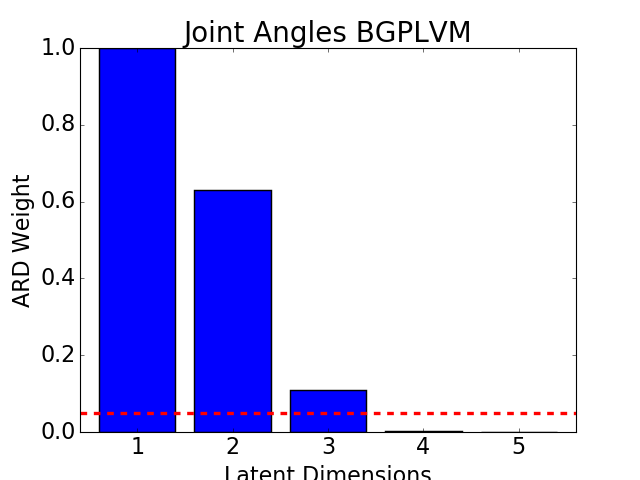
\includegraphics[width=0.3\textwidth]{latentscales.png}
  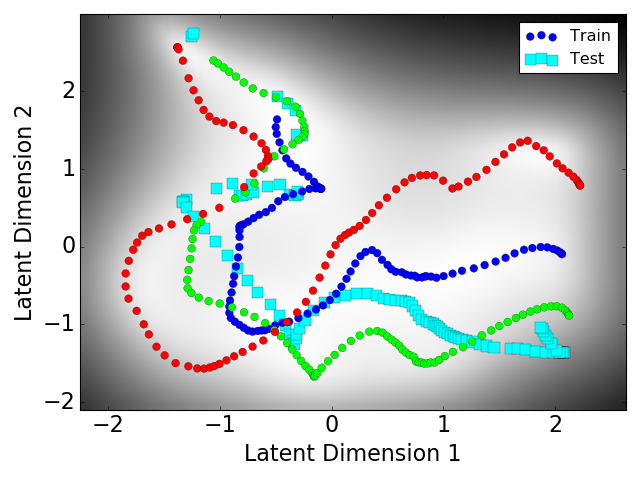
\includegraphics[width=0.3\textwidth]{latentspace.png}
  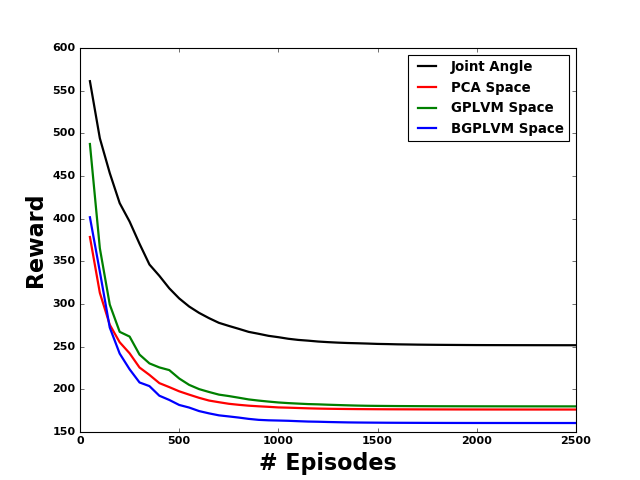
\includegraphics[width=0.3\textwidth]{rlcurve.png}
  \caption{Experimental results of applying BGPLVM to clothing assistance demonstrations for the joint angle scenario. Figure on left shows the resultant ARD weight parameters, figure in the middle shows the latent space and figure on the right shows the learning curves comparing reinforcement learning in latent space and action space.}
  \label{figure:results}
\end{figure}

In this section, we present the applicability of BGPLVM for encoding clothing skills. We used an evaluation dataset given by successful clothing assistance demonstrations for 4 different postures of the mannequin obtained by changing the elevation of the mannequin's arms. Latent spaces were trained by considering 3 trajectories as the training data and the remaining trajectory was used as test data. The ARD weights on training resulted in 3 active latent dimensions for the joint angle scenario and 2 latent dimensions for the end effector scenario. This implies that the motor skills encoded varies depending the input action space. The latent scales and latent space visualizations for the joint angle scenario is shown in Figure~\ref{figure:results}.

Cursor control on the latent space was able to reproduce the clothing demonstration even when the latent trajectory was different from the training latent points. The resultant latent dimensions further captured a specific aspect of the clothing motor-skills. For example, the most significant dimension captured the horizontal motion of the arms along the mannequin while maintaining the constraints for clothing. The second dimension captured various vertical motions of pulling up the T-shirt in the beginning and pulling it down along the torso at the end. A video demonstration of the controller is available at (youtube link).

We further demonstrate the effectivity of performing policy search in the BGPLVM latent space by comparison with search in the high-dimensional action space. For the comparison, the policy search method, policy representation and reward function are the same for both the cases. The main difference is the search space i.e. low-dimensional latent space or high-dimensional action space. CEM was run for 50 iterations where 50 rollouts were performed in each iteration and the top 5 rollouts were retained for computing the mean and variance of the policy parameters. Figure~\ref{figure:results} show the learning curves for both reinforcement learning formulations indicating the latent space scenario outperforms policy search in the high dimensional space, thereby validating our hypothesis.

\section{Conclusion}
\label{section:conclusion}

Motor-skills learning for robotic clothing assistance task involves a high dimensional kinematic search space and maintaining several task space constraints. In this study, we have presented the use of Bayesian Gaussian Process Latent Variable Model (BGPLVM) as a representation for encoding motor-skills to perform clothing assistance task. The experimental results indicate our method as a promising approach in combination with reinforcement learning. There can be several extensions to this work. A latent space representation can be learned from multiple observation spaces using Manifold Relevance Determination (MRD)~\cite{mrd} which is an extension of BGPLVM. Based on this flexibility, our future work will be to learn models that explicitly incorporates visual information of the relationship between the human and cloth. The long term goal is to develop a data-efficient policy search reinforcement learning framework that unifies learning the latent space simultaneously with policy learning.

\section*{Acknowledgement}
This work was supported in part by ImPACT Program of Council for Science, Technology and Innovation (Cabinet Office, Government of Japan) 2015-PM07-36-01. This work was also supported in part by the Grant-in-Aid for Scientific Research from Japan Society for the Promotion of Science (No. 16H01749).

\small

\begin{thebibliography}{15}
\bibitem{tamei}
T. Tamei, T. Matsubara, A. Rai, and T. Shibata, ``Reinforcement Learning of Clothing Assistance with a Dual-arm Robot'' in Proc. of the IEEE-RAS Intl. Conf. on Humanoid Robots (Humanoids), 2011.

\bibitem{bgplvm}
Titsias, M. K., and Lawrence, N. D, ``Bayesian Gaussian process latent variable model'' in Proc. of the Intl. Conf. on Artificial Intelligence and Statistics, 2010.

\bibitem{bitzer}
Bitzer, S., Howard, M., and Vijayakumar, S, ``Using dimensionality reduction to exploit constraints in reinforcement learning'' in Proc. of the IEEE Intl. Conf. on Intelligent Robots and Systems (IROS), 2010.

\bibitem{luck}
Luck, K. S., Neumann, G., Berger, E., Peters, J., and Ben Amor, H, ``Latent space policy search for robotics'' in Proc. of the IEEE Intl. Conf. on Intelligent Robots and Systems (IROS), 2014.

\bibitem{dmp}
Ijspeert, A. J., Nakanishi, J., Hoffmann, H., Pastor, P., and Schaal, S., ``Dynamical movement primitives: learning attractor models for motor behaviors'', in Neural computation 25, no. 2 (2013): 328-373.

\bibitem{lwr}
Schaal, S., and Atkeson, C. G., ``Constructive incremental learning from only local information'', in Neural computation 10.8 (1998): 2047-2084.

\bibitem{via}
Wada, Y., and Kawato, M., ``A theory for cursive handwriting based on the minimization principle'', in Biological Cybernetics 73.1 (1995): 3-13.

\bibitem{mrd}
Damianou, A., Ek, C., Titsias, M., and Lawrence, N, ``Manifold relevance determination'' in Proc. of the Intl. Conf. on Machine Learning, 2012.

\end{thebibliography}

\end{document}
